\documentclass[12pt]{article}
\usepackage[english]{babel}
\usepackage[utf8x]{inputenc}
\usepackage{amsmath}
\usepackage{graphicx}
\setlength {\marginparwidth }{2cm}
\usepackage[colorinlistoftodos]{todonotes}
\usepackage[cyr]{aeguill}
\usepackage[center]{caption}
\usepackage{url}
\usepackage{lipsum}
\usepackage{float}
\usepackage{hyperref}
\usepackage{changepage}
\restylefloat{table}
\setcounter{tocdepth}{5}
\setcounter{secnumdepth}{5}
\usepackage{indentfirst}
\usepackage{subcaption}
\hbadness=99999
\usepackage{algorithm}
\usepackage{algorithmic}
\usepackage{listings}
\lstset
{
    breaklines=true,
    breakatwhitespace=true,
    frame=lines,
    columns=fullflexible,
    basicstyle=\ttfamily,
}

\begin{document}

\begin{titlepage}

\newcommand{\HRule}{\rule{\linewidth}{0.5mm}} % Defines a new command for the horizontal lines, change thickness here

\center % Center everything on the page
 
%----------------------------------------------------------------------------------------
%	HEADING SECTIONS
%----------------------------------------------------------------------------------------

\textsc{\LARGE Université Libre de Bruxelles}\\[1.5cm] % Name of your university/college
\textsc{\Large INFO-H417 : Database System Architecture}\\[0.5cm] % Major heading such as course name
\textsc{\large Project}\\[0.5cm] % Minor heading such as course title

%----------------------------------------------------------------------------------------
%	TITLE SECTION
%----------------------------------------------------------------------------------------

\HRule \\[0.4cm]
{ \huge \bfseries Algorithms in Secondary Memory}\\[0.4cm] % Title of your document
\HRule \\[1.2cm]
 
%----------------------------------------------------------------------------------------
%	AUTHOR SECTION
%----------------------------------------------------------------------------------------

\begin{minipage}{0.8\textwidth}
\begin{flushleft} \large
\emph{Authors:}\\
Soufiane \textsc{AJOUAOU} 000459811\\% Your name
Yahya \textsc{BAKKALI} 000445166\\
Maxime \textsc{HAUWAERT} 000461714
\end{flushleft}
\end{minipage}
~
\begin{minipage}{0.4\textwidth}
\begin{flushright} \large
\end{flushright}
\end{minipage}\\[2cm]

% If you don't want a supervisor, uncomment the two lines below and remove the section above
%\Large \emph{Author:}\\
%John \textsc{Smith}\\[3cm] % Your name

%----------------------------------------------------------------------------------------
%	DATE SECTION
%----------------------------------------------------------------------------------------

{\large \today}\\[1cm] % Date, change the \today to a set date if you want to be precise

%----------------------------------------------------------------------------------------
%	LOGO SECTION
%----------------------------------------------------------------------------------------


\includegraphics[width=4.3cm, height=4.3cm]{sceau-a-quadri.jpg}\\%% Include a department/university logo - this will require the graphicx package
 
%----------------------------------------------------------------------------------------

\vfill % Fill the rest of the page with whitespace

\end{titlepage}

\tableofcontents
\newpage

\section{Introduction and Environment}
\subsection{Introduction}
%Briefly summarize the project goals.
The goal of this project is to compare the performance of different methods for reading and writing to secondary memory by using them in different algorithms.\\

Four methods will be implemented, one that uses one character at a time, one using a buffering mechanism, one that uses a buffer of a predefined size and one using memory mapping.\\

Four algorithms will be implemented, one that reads the file and computes the sum of the lengths of each line of a file, one that reads randomly the file and computes the lengths of the next lines, one that merges different files and one that sorts a file.\\

In this report, the implementations of the different methods will be seen then all the results will be shown and discussed.
% Can be more developed if needed
\subsection{Environment}
%Document the machine environment on which the experiments were run (mentioning disk type, amount of memory, etc); the programming language used; and the external libraries used (if any).

Here are the specifications of the computer used for the benchmark :
\begin{itemize}
    \item CPU : Intel Core i7-8750H
    \item RAM : 8GB DDR4, 2400Mhz
    \item Memory : 480 GB SSD with 540 MB/s read speed and 555 MB/s write speed
    \item Operating system : Ubuntu 20
\end{itemize}

The programming language used for this project was Java 13.\\

The following external libraries have been used :
\begin{itemize}
    \item JMH : It has been used to easily make benchmarks.
    \item Junit : It has been used to test the different implementations.
\end{itemize}

\subsection{Definitions}
For the different implementations, a notation will be used and it is as follows :
\begin{itemize}
    \item One refers to the first implementation.
    \item Buffered refers to the second implementation.
    \item OneBuffer refers to the third implementation.
    \item MMap refers to the fourth implementation.
\end{itemize}

To estimate the costs the following parameters will be used :
\begin{itemize}
    \item B(R) : The number of blocks that R occupies on disk.
    \item B($l_i$) : The number of blocks that a line $i$ occupies on disk.
    \item S : The number of main memory buffers available.
    \item D : The default buffer size of the Buffered implementation and it is equal to 8 kB based on its source code. 
\end{itemize}
\section{Observations on reading and writing}
\subsection{Implementation}
%For each of the 4 implementations, briefly explain the implementation in your own words. Give details on how you programmed the implementation if necessary.

The figure \ref{fig:1} shows an UML diagram describing the structure of the implementation:

\begin{figure}[H] 
\begin{adjustwidth}{-3cm}{-1cm}
 \begin{center}
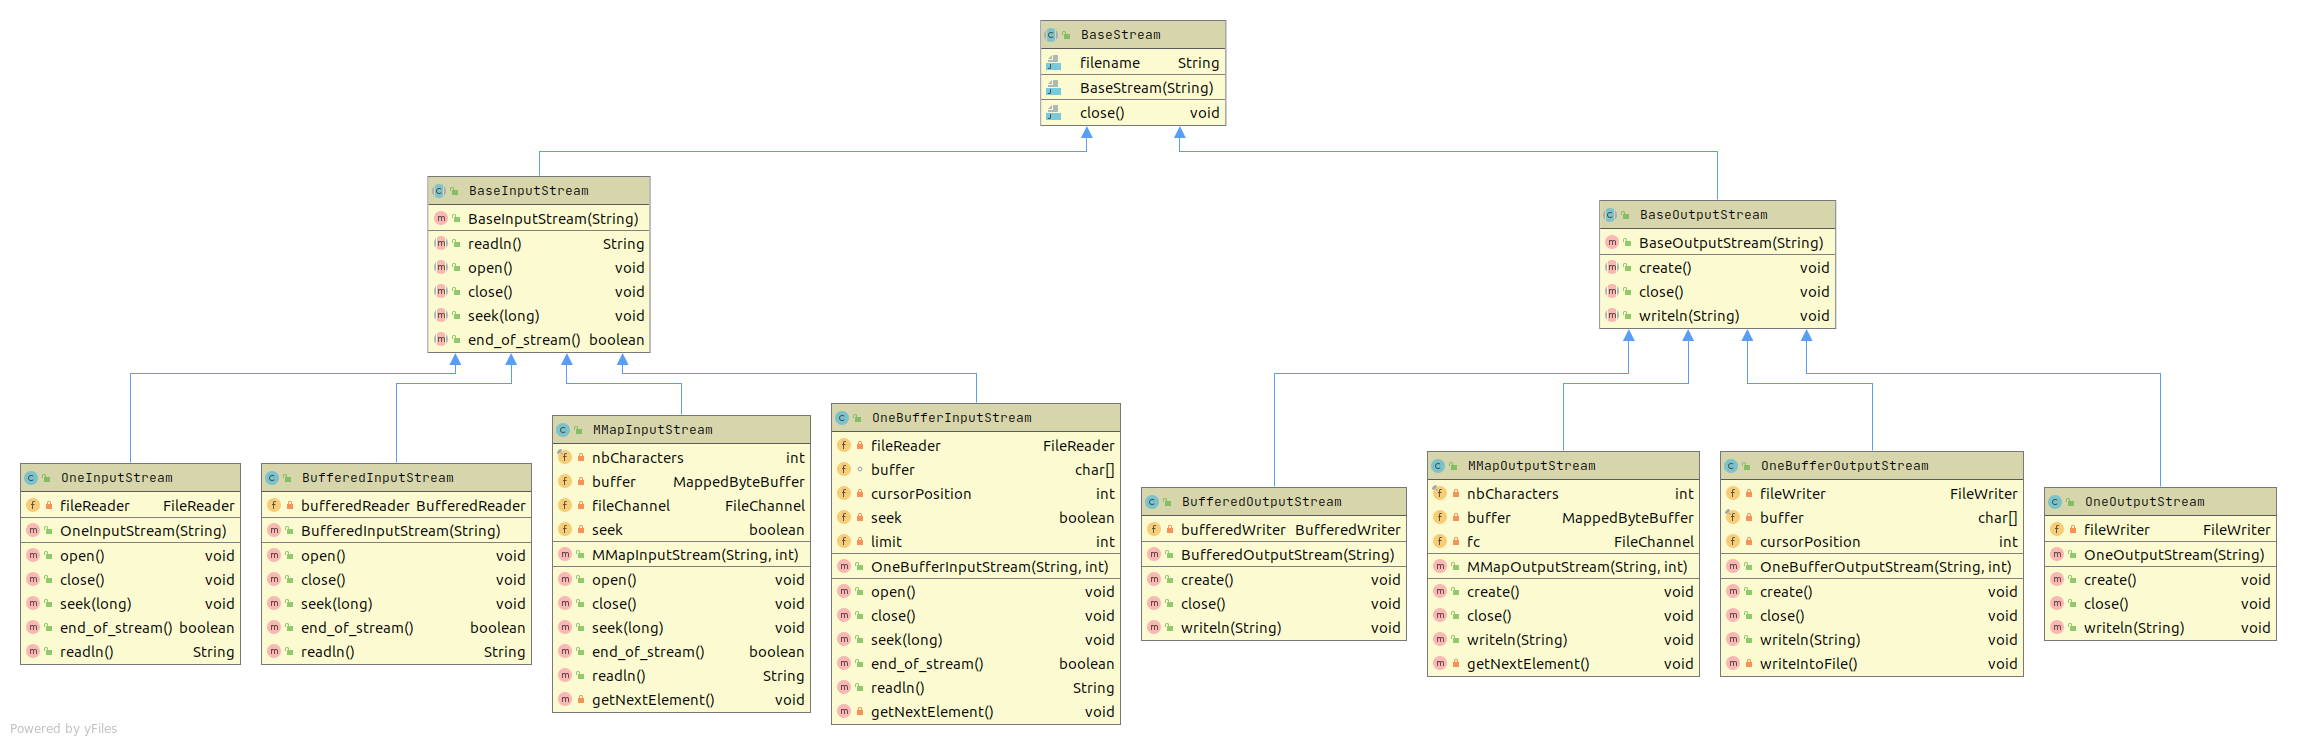
\includegraphics[width=20cm]{images/Stream.png}
\end{center}
\caption{Stream structure}
\label{fig:1}
\end{adjustwidth}
\end{figure}

In order to facilitate the use of different implementations, it is useful to use abstract classes. In addition, a factory model has been introduced via different classes such as BaseStream, Generator and BaseAlgo. The purpose of using this type of methodology is to avoid code duplication and to obtain a generic code. This type of class allows us to instance abstract classes without knowing the type of the abstract class.

For the different implementations, the open/create and close methods are basic : they simply create a new object instance, close the stream and free all the system resources associated with it. For all implementations other than MMap, there is no predefined method to seek in the file. 

To do this, the procedure chosen was as follows :
\begin{itemize}
    \item Close the current stream
    \item Re-open the stream
    \item Skip n position
\end{itemize}

The \texttt{readln} and the \texttt{writeln} of each of these implementations will be explained in the following sections.

\subsubsection{One}
This method reads and writes the files byte by byte. It has a \texttt{FileReader} attribute.
\begin{itemize}
    \item readln : It works by calling multiple times the \texttt{read} method of its \texttt{fileReader}. Each time the method is called, the type of the character read is verified, if it is an \texttt{end-of-line} or an \texttt{end-of-stream} the method returns the string else the character is added to the string.

    \item writeln : It works by calling the \texttt{write} method of its \texttt{fileReader} multiple times. Each character of the specified string is written in the file with the method. Then an \texttt{end-of-line} character is added.

\end{itemize}

\begin{algorithm}[H]
\caption{readln}
\label{algo:1}
\begin{algorithmic}[1]
\IF {end of stream}
\RETURN null
\ELSE
\STATE {Create an empty line to store the next line}
\STATE {Read the first character}
\WHILE{the character is not an end of line or end of stream}
\STATE {Add the character to the line}
\STATE {Read the next character}
\ENDWHILE
\RETURN the line
\ENDIF
\end{algorithmic}
\end{algorithm}

\begin{algorithm}[H]
\caption{writeln}
\label{algo:2}
\begin{algorithmic}[1]
\FOR{each character in the line}
\STATE {Write the character and flush it into the file}
\ENDFOR
\STATE {Write the end of line character and flush it into the file}
\end{algorithmic}
\end{algorithm}

\subsubsection{Buffered}
This method reads and writes the files with a predefined buffering mechanism. It has a \texttt{BufferedReader} that is wrapped around a \texttt{FileReader}.

\begin{itemize}
    \item readln : This method just return the result of the call of the method \texttt{readLine()} of its \texttt{bufferedReader}.
    
    \item writeln : The \texttt{writeln} method just calls the method \texttt{write()} of its \texttt{bufferedReader} with the specified string with an \texttt{end-of-line} at the end.
\end{itemize}

\begin{algorithm}[H]
\caption{readln}
\label{algo:3}
\begin{algorithmic}[1]
\RETURN the line returned by the \texttt{readLine()} method
\end{algorithmic}
\end{algorithm}

\begin{algorithm}[H]
\caption{writeln}
\label{algo:4}
\begin{algorithmic}[1]
\STATE {Write the line with end of line character and flush them into the file}
\end{algorithmic}
\end{algorithm}

\subsubsection{OneBuffer}
This method reads and writes the files with a buffer of a predefined size B.

\begin{itemize}
    \item readln : For each character of the buffer its type is verified, if it is an \texttt{end-of-line} or an \texttt{end-of-stream} the method returns the string, else the character is added to the string. When the buffer is empty, it is filled with a call of the \texttt{read} method of its \texttt{fileReader} that reads at the maximum B characters.
    
    \item writeln : While there are still characters to write, the buffer is filled with the next characters and they are written to the file with a call of the \texttt{write} method of its \texttt{fileReader} then adds an \texttt{end-of-line} at the end.
\end{itemize}

\begin{algorithm}[H]
\caption{readln}
\label{algo:5}
\begin{algorithmic}[1]
\IF {end of stream}
\RETURN null
\ELSE
\STATE {Create an empty line to store the next line}
\WHILE{the character is not an end of line or end of stream}
\IF {Cursor position exceeds buffer size}
\STATE {Read the next B character(s) from the file}
\STATE {Set the cursor position to zero}
\ENDIF
\STATE {Read the character from the buffer at the cursor position}
\STATE {Add the character to the line}
\STATE {Increment cursor position}
\ENDWHILE
\RETURN the line
\ENDIF
\end{algorithmic}
\end{algorithm}

\begin{algorithm}[H]
\caption{writeln}
\label{algo:6}
\begin{algorithmic}[1]
\FOR{each character in the line}
\IF {cursor position exceeds buffer size}
\STATE {Write the next B character(s) and flush it into the file}
\STATE {Set the cursor position to zero}
\ENDIF
\STATE {Add the character to the buffer at the cursor position}
\STATE {Increment cursor position}
\ENDFOR
\STATE {Add the end of line character to the buffer at the cursor position}
\STATE {Increment cursor position}
\end{algorithmic}
\end{algorithm}

\subsubsection{MMap}

\paragraph{Concept}\mbox{}\\ \par

Memory mapping allows you to assign directly byte by byte a part of the file. The file must be present on the disk or on a device accessible from a file descriptor. This allows us to directly manipulate mapped portions of the file through a pointer.  Writing or reading the file becomes as much simple as manipulating data from a variable. The advantage of this method is that it is not linked to RAM unlike the most common I/O methods. It is also advantageous for large files as the memory mapping allows to access specific areas of the file quite fast. A file can also be mapped by several applications simultaneously. 

\paragraph{Methods}\mbox{}\\ \par
This method reads and writes the files by memory mapping. It maps a part of a file into a memory. It allows the program to modify this part of a file like a basic object in the dynamic memory.

\begin{itemize}
    \item readln : For each element of the buffer its type is verified, if it is an \texttt{end-of-line} or an \texttt{end-of-stream} the function returns the string else it is added to the string. When the buffer is empty, it is filled thanks to a call of the \texttt{map} method of its \texttt{fileChannel}, it maps the next B characters. The use of a \texttt{ByteArrayOutputStream} object was needed in order to support special characters, such as ó.
    
    \item writeln : While there are still characters to write, the buffer is filled with the next characters and they are written to the file with a call of the \texttt{put} method. When the buffer is full it is replaced by the new buffer of the next mapped part.
\end{itemize}

\begin{algorithm}[H]
\caption{readln}
\label{algo:7}
\begin{algorithmic}[1]
\IF {end of stream}
\RETURN null
\ELSE
\STATE {Create an empty line to store the next line}
\WHILE{the character is not an end of line or end of stream}
\IF {the buffer has no remaining characters}
\STATE {Map the next B character(s) from the file}
\ENDIF
\STATE {Get the character from the mapped buffer}
\STATE {Add the character to the line}
\ENDWHILE
\RETURN the line
\ENDIF
\end{algorithmic}
\end{algorithm}

\begin{algorithm}[H]
\caption{writeln}
\label{algo:8}
\begin{algorithmic}[1]
\FOR{each character in the line}
\IF {the mapped buffer size has been exceeded}
\STATE {Map the next B character(s)}
\ENDIF
\STATE {Put the character into the mapped buffer}
\ENDFOR
\STATE {Put the end of line character into the mapped buffer}
\end{algorithmic}
\end{algorithm}

\subsection{Experiment 1.1} \label{exp1.1}
\subsubsection{Discussion}
%Discuss the expected behavior, cost formulas, and what you observe during your experiments.
The sequential reading is an algorithm that reads sequentially the specified file and computes the sum of the length of all the lines.

It has a cost that depends on the cost of \texttt{readln} on the entire file of the method used.

\begin{itemize}
    \item One : The cost expected is equal to $B(R)$ I/O operations, as it reads the file byte by byte.
    \item Buffered : The cost expected is equal to $\lceil\frac{B(R)}{D}\rceil$ I/O operations \footnotemark.
    \item OneBuffer : The cost expected is equal to $\lceil\frac{B(R)}{S}\rceil$ I/O operations. As each time the reading is done from the buffer and not from the disk \footnotemark[\value{footnote}], until the buffer becomes empty then an I/O operation is performed to refill it.
    \item MMap : The cost expected is the same as the OneBuffer but as described in its JavaDoc ``mapping a file into memory is more expensive than reading or writing a few tens of kilobytes of data via the usual read and write methods" so the cost can be more than expected.
\end{itemize}
\footnotetext{$\mathcal{O}(n)$, n refers the buffer size, will be ignored}

After estimating the cost, an implementation ranking can be made for the expected results. First it is expected that the OneBuffer is the best, then the Buffered followed by the MMap and lastly the One.

\subsubsection{Experimental observations} \label{res1.1}
Before comparing different implementations, it is necessary to determine the optimal buffer size for the implementations that use it. In order to use it at its full power. For all the benchmarks of this experiment, the parameters were set to 1 iteration of warmup and 3 iterations of measurement. The average time will be calculated in seconds
%Use graphs and plots to compare the implementations.
\paragraph{Optimal buffer size values}\mbox{}\\
\par The benchmark was run on values belonging to three different scales.
\begin{center}
\begin{tabular}{|c|c|}
\hline
\textbf{Scale} & \textbf{Value}\\
\hline\hline
Bytes & 16, 256 \\
\hline
kB & 4, 64, 256, 512, 750 \\
\hline
MB & 1, 4, 16 \\
\hline
\end{tabular}
\end{center}

For OneBuffer implementation, the file chosen for the benchmark was ``cast\_info.csv"; its size is almost 1,4 GB. Depending on the results of the benchmark analysis in the figure \ref{fig:2a}, increasing the buffer size at a certain point can speed up the execution time but exceeding it afterwards can make it worse again. For the upcoming length programs benchmarking, the buffer size is set to 750 kB.

For MMap implementation, the file chosen for the benchmark was ``keyword.csv"; its size is almost 4 MB. Depending on the results of the benchmark analysis in the figure \ref{fig:2b}, all values may be optimal except 16 Byte which is slower. To verify this, further benchmarking tests were carried on other files and for each of them, the different buffer sizes neither increase nor decrease the speed because they have almost identical execution time. To keep the same size as the OneBuffer implementation the buffer size is also set to 750 kB.

\begin{figure}[H] 
\begin{adjustwidth}{-3.5cm}{-3.5cm}
  \begin{subfigure}[b]{0.5\linewidth}
    \centering
    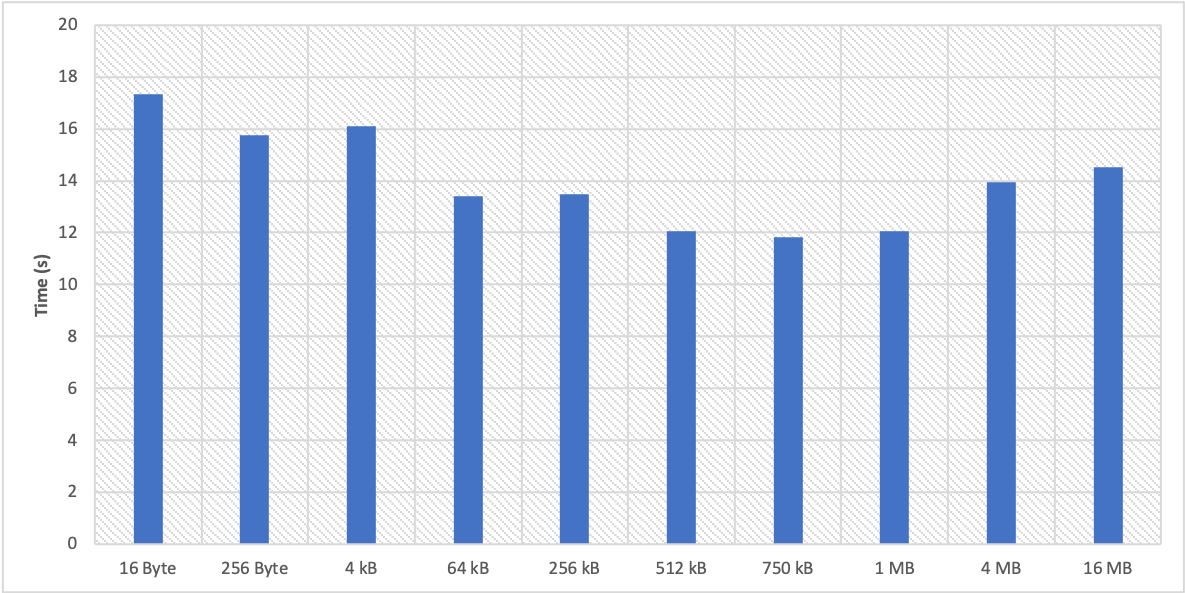
\includegraphics[width=0.99\linewidth]{images/oneBuffer-length.png} 
    \caption{OneBuffer} 
    \label{fig:2a} 
    \vspace{4ex}
  \end{subfigure}%% 
  \begin{subfigure}[b]{0.5\linewidth}
    \centering
    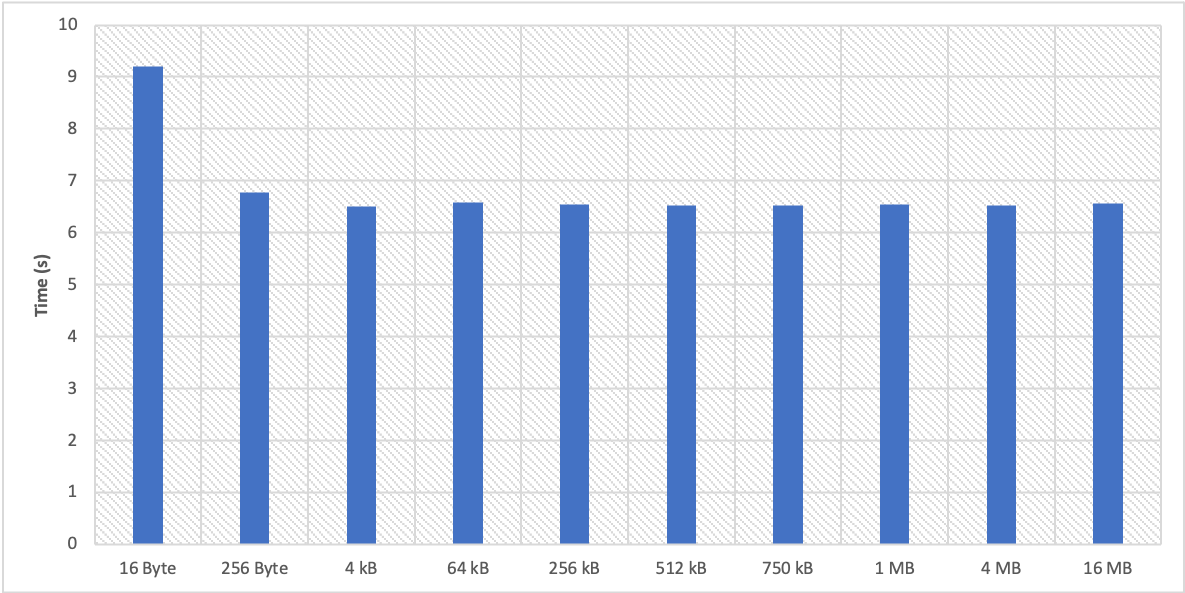
\includegraphics[width=0.99\linewidth]{images/MMap-length.png} 
    \caption{MMap} 
    \label{fig:2b} 
    \vspace{4ex}
  \end{subfigure} 
  \caption{Buffer size parameter tuning}
  \label{fig:2} 
\end{adjustwidth}
\end{figure}
\paragraph{Files benchmark}\mbox{}\\
\par The benchmark was performed on all files, except for the MMap implementation where the execution time started to increase and become important at some point. Also, the buffer size has been set to 750 kB for OneBuffer and MMap. The table below shows the obtained values.

\begin{table}[H]
\begin{tabular}{|l|l|l|l|l|}
\hline
                     & One    & Buffered & OneBuffer & Mmap   \\ \hline
Files                & \multicolumn{4}{c|}{Units (s/op)}      \\ \hline
comp\_cast\_type.csv & 0,001  & 0,0001   & 0,001     & 0,001  \\ \hline
kind\_type.csv       & 0,001  & 0,0001   & 0,001     & 0,001  \\ \hline
company\_type.csv    & 0,001  & 0,0001   & 0,001     & 0,001  \\ \hline
role\_type.csv       & 0,001  & 0,0001   & 0,001     & 0,001  \\ \hline
link\_type.csv       & 0,001  & 0,0001   & 0,001     & 0,001  \\ \hline
info\_type.csv       & 0,001  & 0,001    & 0,001     & 0,003  \\ \hline
movie\_link.csv      & 0,042  & 0,007    & 0,016     & 0,671  \\ \hline
complete\_cast.csv   & 0,16   & 0,019    & 0,03      & 2,36   \\ \hline
keyword.csv          & 0,247  & 0,031    & 0,056     & 3,579  \\ \hline
company\_name.csv    & 1,059  & 0,129    & 0,221     & 15,898 \\ \hline
movie\_info\_idx.csv & 2,094  & 0,196    & 0,371     & 32,994 \\ \hline
aka\_title.csv       & 1,627  & 0,297    & 0,55      & 34,448 \\ \hline
aka\_name.csv        & 3,148  & 0,363    & 0,882     & 64,66  \\ \hline
movie\_companies.csv & 3,148  & 0,5      & 0,981     & 85,379 \\ \hline
movie\_keyword.csv   & 4,058  & 0,583    & 1,012     & 88,95  \\ \hline
title.csv            & 8,486  & 1,338    & 2,489     &        \\ \hline
char\_name.csv       & 7,71   & 1,569    & 2,752     &        \\ \hline
name.csv             & 11,168 & 2,011    & 4,147     &        \\ \hline
person\_info.csv     & 13,424 & 1,908    & 3,863     &        \\ \hline
movie\_info.csv      & 33,935 & 3,469    & 8,641     &        \\ \hline
cast\_info.csv       & 51,614 & 5,256    & 11,751    &        \\ \hline
\end{tabular}
\end{table}

To facilitate the reading of the result obtained, the figure \ref{fig:3} groups together these four implementations and their execution times.

\begin{figure}[H] 
\begin{adjustwidth}{-3cm}{-1cm}
 \begin{center}
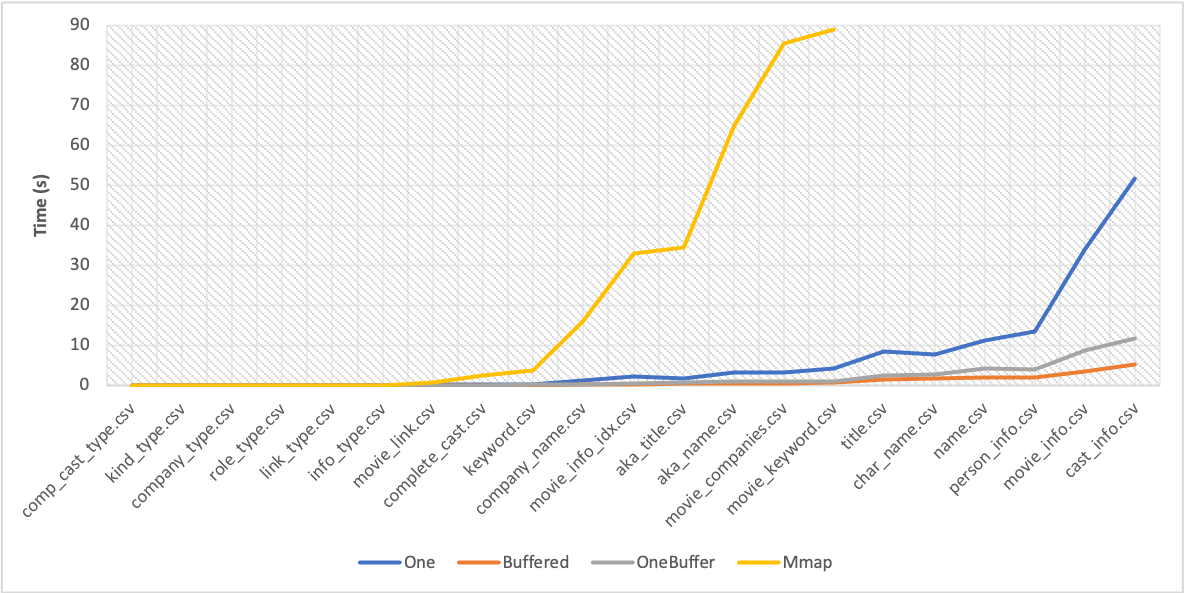
\includegraphics[width=20cm]{images/length.png}
\end{center}
\caption{Length program execution time}
\label{fig:3}
\end{adjustwidth}
\end{figure}
\subsubsection{Explanation}
%Explain what you observe.
The ranking obtained does not follow the expected one. Because the Buffered is the best and not the OneBuffer. The choice of the OneBuffer was made because both use a memory buffer but the size of the OneBuffer is too big. The performances are quite close, so this difference is explained by the fact that the Buffered is well developed by java and optimized to the maximum. The other difference is that the One was better than the MMap, the reason why the MMap expected to be more performant is that it has a buffer in memory but as said in JavaDoc the simple reading can be better for small files and also the manual management of the UTF8 encoding for the MMap can also increase the execution time.
\subsection{Experiment 1.2} \label{exp1.2}
\subsubsection{Discussion}
%Discuss the expected behavior, cost formulas, and what you observe during your experiments.
The random reading is an algorithm that randomly jumps, $j$ times, to a position in the specified file and reads the next line from that position and calculates the sum of the length of all lines read.  Its cost depends on the value of $j$ and the cost of \texttt{seek} and \texttt{readln} of the method used.

As explained earlier, there is no predefined seek method for the One, Buffered and OneBuffer implementations. Therefore, an approach was followed to create it. The chosen method was too expensive because it is not executed as an atomic operation like the MMap. As three steps are necessary, first the stream must be closed, then it must be reopened so that the cursor can be placed at the beginning of the file stream and finally a certain number of bytes must be skipped to position the cursor at the desired location. The estimated cost for this block of operation is as follows :
\begin{itemize}
    \item Close : release the resources + free the buffer \footnotemark.
    \item Reopen : allocate the resources + an-in memory buffer \footnotemark[\value{footnote}].
    \item Skip n bytes : 1 I/O operation + fill the buffer \footnotemark[\value{footnote}].
\end{itemize}
\footnotetext{Does not apply for the One implementation}
On the other hand the MMap uses a \texttt{FileChannel} method that allows to move the cursor and read from any position directly.

\begin{itemize}
    \item Seek\footnote{Consider only the I/O cost} :
    \begin{itemize}
        \item One : The cost expected is equal to $j$ I/O operations.
        \item OneBuffer : The cost expected is equal to $j$ I/O operations.
        \item Buffered : The cost expected is equal to $j$ I/O operations.
        \item MMap : The cost expected is equal to 0 I/O operations.
    \end{itemize}
    
    \item readln :
    \begin{itemize}
        \item One : The cost expected is equal to $\sum_{i=0}^{j} B(l_i)$ I/O operations.
        \item OneBuffer : The cost expected is equal to $\sum_{i=0}^{j} \lceil\frac{B(l_i)}{D}\rceil$ I/O operations.
        \item Buffered : The cost expected is equal to $\sum_{i=0}^{j} \lceil\frac{B(l_i)}{S}\rceil$ I/O operations.
        \item MMap : The cost expected is equal to $\sum_{i=0}^{j} \lceil\frac{B(l_i)}{S}\rceil$ I/O operations.
    \end{itemize}
\end{itemize}

The estimated overall cost is as follows :

\begin{center}
\begin{tabular}{|c|c|}
\hline
\textbf{Implementation} & \textbf{Cost (I/O operation)}\\
\hline\hline
One & $j + \sum_{i=0}^{j} B(l_i)$\\
[5pt]\hline
Buffered &  $j + \sum_{i=0}^{j} \lceil\frac{B(l_i)}{D}\rceil$\\
[5pt]\hline
OneBuffer & $j + \sum_{i=0}^{j} \lceil\frac{B(l_i)}{S}\rceil$\\
[5pt]\hline
MMap & $\sum_{i=0}^{j} \lceil\frac{B(l_i)}{S}\rceil$\\
[5pt]\hline
\end{tabular}
\end{center}

After estimating the cost, an implementation ranking can be made for the expected results. First it is expected that the MMap is the best, then the One followed by the Buffered and lastly the OneBuffer.

\subsubsection{Experimental observations} \label{res1.2}
%Use graphs and plots to compare the implementations.
The benchmark was realized using four j-values which are 10, 100, 1000 and 10000. For the sub-benchmarks 10 and 100 all files were tested, except for the sub-benchmarks 1000 and 10000 where the execution time started to increase and become important after a certain file size. In addition, the buffer size was set to 750 kB for OneBuffer and MMap as for the first experiment. Figure \ref{fig:4} groups these four sub-benchmarks and their execution times. 

\begin{figure}[H] 
\begin{adjustwidth}{-3.5cm}{-3.5cm}
  \begin{subfigure}[b]{0.5\linewidth}
    \centering
    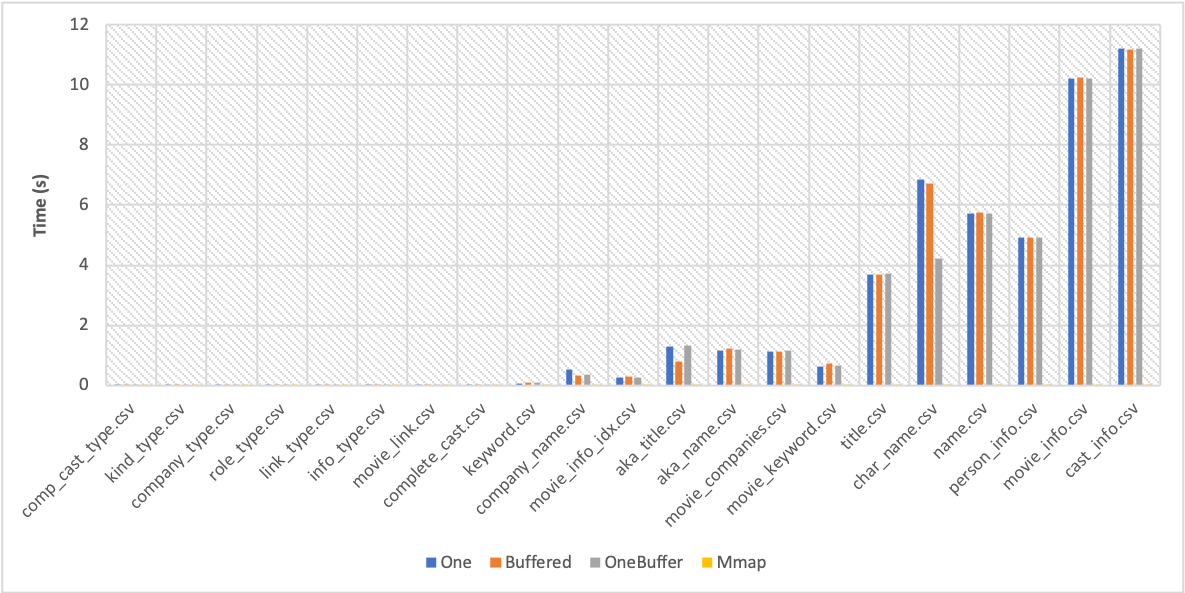
\includegraphics[width=0.99\linewidth]{images/randjump-10.png} 
    \caption{j = 10} 
    \label{fig:4a} 
    \vspace{4ex}
  \end{subfigure}%% 
  \begin{subfigure}[b]{0.5\linewidth}
    \centering
    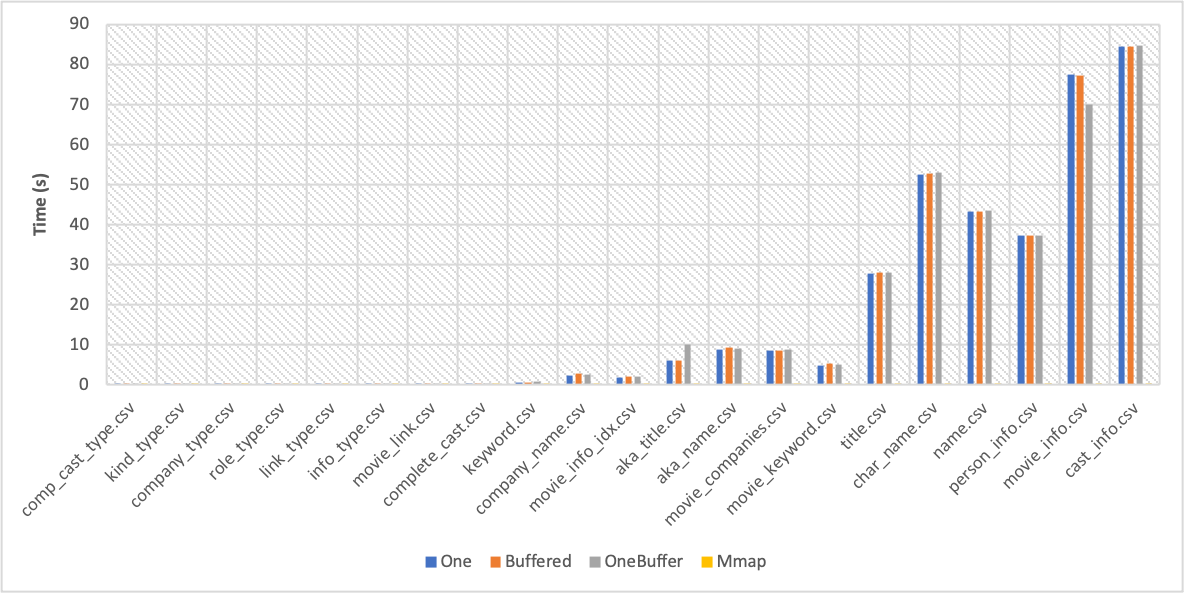
\includegraphics[width=0.99\linewidth]{images/randjump-100.png} 
    \caption{j = 100} 
    \label{fig:4b} 
    \vspace{4ex}
  \end{subfigure} 
  \begin{subfigure}[b]{0.5\linewidth}
    \centering
    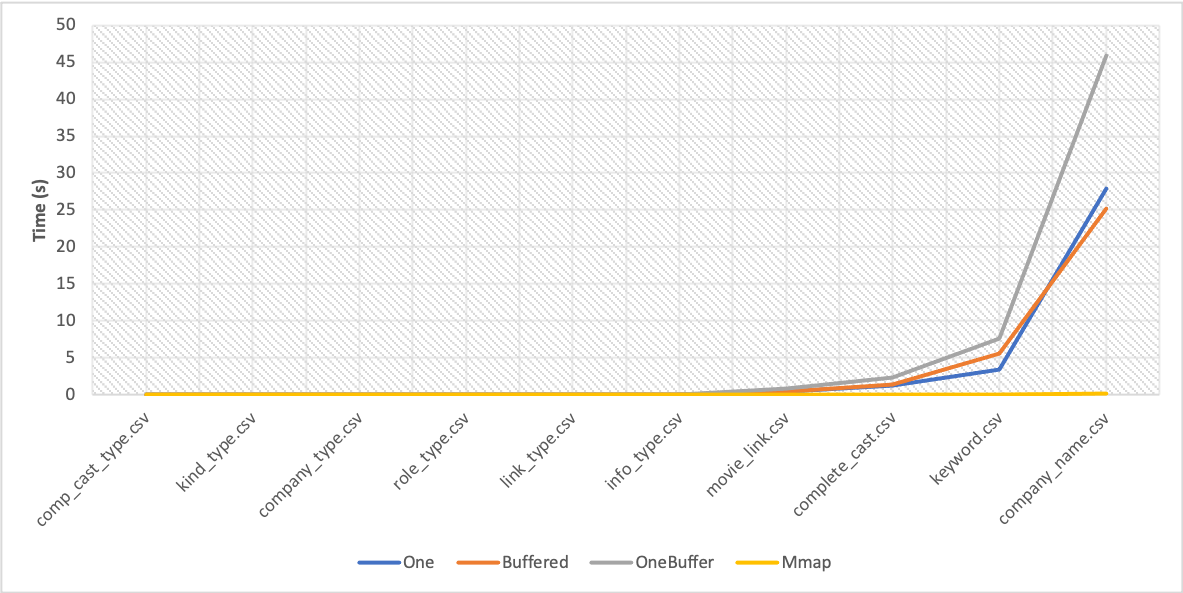
\includegraphics[width=0.99\linewidth]{images/randjump-1000.png} 
    \caption{j = 1000} 
    \label{fig:4c} 
  \end{subfigure}%%
  \begin{subfigure}[b]{0.5\linewidth}
    \centering
    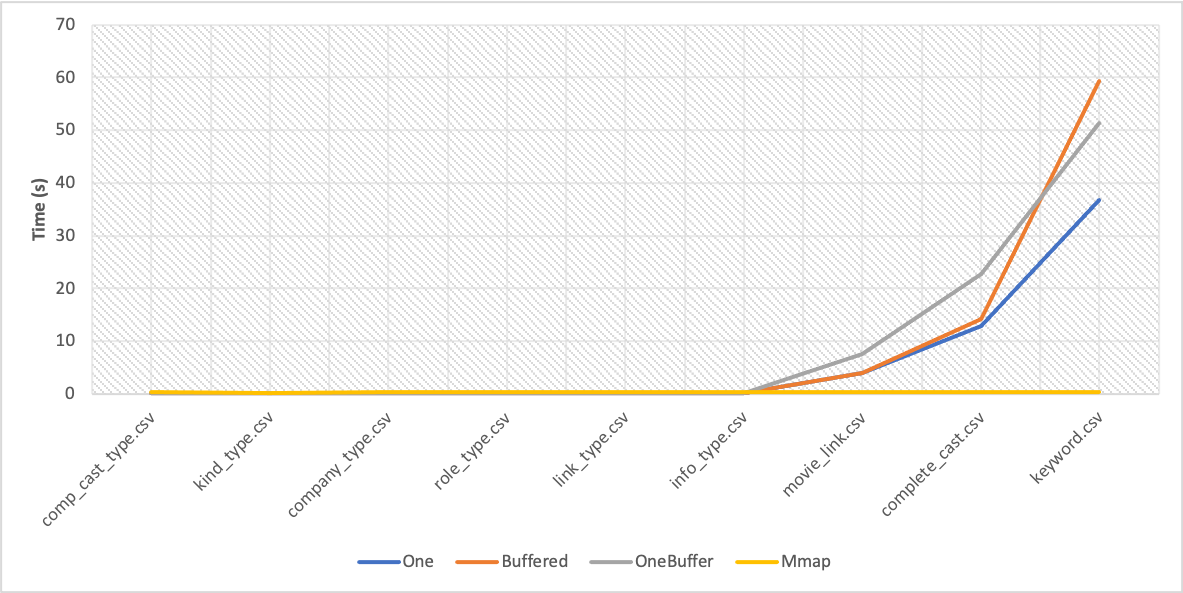
\includegraphics[width=0.99\linewidth]{images/randjump-10000.png} 
    \caption{j = 10000} 
    \label{fig:4d} 
  \end{subfigure} 
  \caption{Randjump program execution on different values j}
  \label{fig:4} 
\end{adjustwidth}
\end{figure}

\subsubsection{Explanation}
%Explain what you observe.
The ranking obtained follows the expected one. MMap has the best performance and far exceeds that of other implementations, even for the largest j and file sizes. For other implementations and a smaller j equals 10 or 100. The difference goes almost unnoticed, on the other hand when the j becomes big the difference starts to dig in as the One remains faster followed by the Buffered and finally the OneBuffer which is well in line with the predictions made, because the ignored costs for the seek start to make the difference.


\subsection{Experiment 1.3} \label{exp1.3}

\subsubsection{Discussion}
%Discuss the expected behavior, cost formulas, and what you observe during your experiments.
The RRMerge is an algorithm that merges the content of all the specified files. The first lines of every files are written in the output file, then the second lines etc., until there are no lines left.

It has a cost that depends on the number and the size of the files to merge, the cost of \texttt{readln} of the input stream used and the cost of \texttt{writeln} of the output stream used.

As the readln has already been seen in the first experiment, only the writeln will be.

\begin{itemize}
    \item One : The cost expected is equal to $B(R)$ I/O operations, as it writes into the file byte by byte.
    \item Buffered : The cost expected is equal to $\lceil\frac{B(R)}{D}\rceil$ I/O operations \footnotemark.
    \item OneBuffer : The cost expected is equal to $\lceil\frac{B(R)}{S}\rceil$ I/O operations. As each time the write is done into the buffer and not the disk \footnotemark[\value{footnote}], until the buffer becomes full then an I/O operation is performed to flush it.
    \item MMap : The cost expected is the same as the OneBuffer but as described in its JavaDoc ``mapping a file into memory is more expensive than reading or writing a few tens of kilobytes of data via the usual read and write methods" so the cost can be more than expected.
\end{itemize}
\footnotetext{$\mathcal{O}(n)$, n refers the buffer size, will be ignored}

The estimated overall I/O operation cost is as follows :

\begin{center}
\begin{tabular}{|c|c|c|}
\hline
\textbf{Implementation} & \textbf{Read} & \textbf{Write}\\
\hline\hline
One & $B(R)$ & $B(R)$\\
[5pt]\hline
Buffered &  $\lceil\frac{B(R)}{D}\rceil$ & $\lceil\frac{B(R)}{D}\rceil$\\
[5pt]\hline
OneBuffer & $\lceil\frac{B(R)}{S}\rceil$ & $\lceil\frac{B(R)}{S}\rceil$\\
[5pt]\hline
MMap & $\lceil\frac{B(R)}{S}\rceil$ & $\lceil\frac{B(R)}{S}\rceil$\\
[5pt]\hline
\end{tabular}
\end{center}

After estimating the cost and on the basis of the \hyperref[res1.1]{results of experience 1.1} and \hyperref[res1.2]{results of experience 1.2}. A top 3 (x,y) pair ranking can be done for the expected results. As the results of experiment 1.1 confirmed that Buffered was too fast compared to MMap and knowing that the same output stream will have the same performance as any input stream, the choice of MMap as input stream can already be eliminated as it will never perform better than Buffered using the same output stream. As for reading, the expected ranking of the writing implementation is as follows. First, the OneBuffer is expected to be the best, then the Buffered, followed by the MMap and finally the One. So the top 3 ranking can be as follows : 
\begin{itemize}
    \item[1] (Buffered, OneBuffer)
    \item[2] (Buffered, Buffered)
    \item[3] (Buffered, MMap)
\end{itemize}

\subsubsection{Experimental observations} \label{res1.3}
%Use graphs and plots to compare the implementations.
For this benchmark, different versions of this algorithm will be created. Each version represents a unique pair (x,y) of implementation of the input stream x and implementation of the output stream y. For the x pair, the best implementation as identified in \hyperref[exp1.1]{experiment 1.1} and the best implementation as identified in \hyperref[exp1.2]{experiment 1.2} have been used, which are Buffered and MMap. For y, all possible implementations have been tested. The files were first sorted in ascending order, then sub-sets were created each time according to the number n chosen. For example, for n = 3 the first 3 small files were taken and merged. The maximum test value was 17, so the files ``name.csv", ``person\_info.csv", ``movie\_info.csv" and ``cast\_info.csv" were not used. The table below shows the obtained values for the different (x,y) pairs merging different file sizes. In addition, the buffer size was set to 512 kB for OneBuffer and MMap. To facilitate the reading of the result obtained, the table has been divided into two figures. Figure \ref{fig:5} groups the buffered input stream with the four output streams and their execution times. On the other hand, the figure \ref{fig:6} groups the MMap input stream with the four output streams and their execution times.

\begin{table}[H]
\tiny
\begin{adjustwidth}{-3.5cm}{-3cm}
\begin{tabular}{|l|l|l|l|l|l|l|l|l|l|l|l|l|l|l|l|l|}
\hline
                      & \multicolumn{5}{c|}{Byte}             & \multicolumn{11}{c|}{MB}                                                                         \\ \hline
Pair                  & 130   & 222   & 382   & 643   & 2691  & 0,7 MB & 3,1    & 6,9    & 24,7   & 60      & 98,9    & 171,9 & 265    & 358,8  & 562,7 & 778,4  \\ \hline
(Buffered, One)       & 0,001 & 0,002 & 0,003 & 0,003 & 0,009 & 1,412  & 6,617  & 14,559 & 52,022 & 128,359 & 209,653 &       &        &        &       &        \\ \hline
(Buffered, Buffered)  & 0,001 & 0,001 & 0,001 & 0,001 & 0,003 & 0,079  & 0,417  & 0,747  & 1,445  & 4,71    & 5,946   & 9,867 & 17,173 & 29,219 & 37,8  & 47,005 \\ \hline
(Buffered, OneBuffer) & 0,001 & 0,001 & 0,001 & 0,001 & 0,002 & 0,014  & 0,044  & 0,096  & 0,363  & 0,819   & 1,413   & 2,617 & 3,666  & 4,988  & 7,983 & 10,174 \\ \hline
(Buffered, Mmap)      & 0,001 & 0,001 & 0,001 & 0,001 & 0,001 & 0,015  & 0,055  & 0,114  & 0,348  & 0,745   & 1,243   & 2,072 & 2,828  & 3,918  & 6,175 & 8,857  \\ \hline
(Mmap, One)           & 0,003 & 0,003 & 0,004 & 0,005 & 0,015 & 2,606  & 12,176 & 26,428 & 93,02  & 231,51  & 375,48  &       &        &        &       &        \\ \hline
(Mmap, Buffered)      & 0,002 & 0,002 & 0,002 & 0,004 & 0,009 & 1,285  & 5,874  & 12,673 & 42,662 & 107,013 & 170,846 &       &        &        &       &        \\ \hline
(Mmap, OneBuffer)     & 0,002 & 0,002 & 0,003 & 0,004 & 0,01  & 1,247  & 5,451  & 11,928 & 41,538 & 102,849 & 166,711 &       &        &        &       &        \\ \hline
(Mmap, Mmap )         & 0,002 & 0,001 & 0,003 & 0,003 & 0,01  & 1,23   & 5,49   & 12,096 & 41,249 & 103,288 & 165,711 &       &        &        &       &        \\ \hline
\end{tabular}
\end{adjustwidth}
\end{table}


\begin{figure}[H] 
\begin{adjustwidth}{-3cm}{-3cm}
 \begin{center}
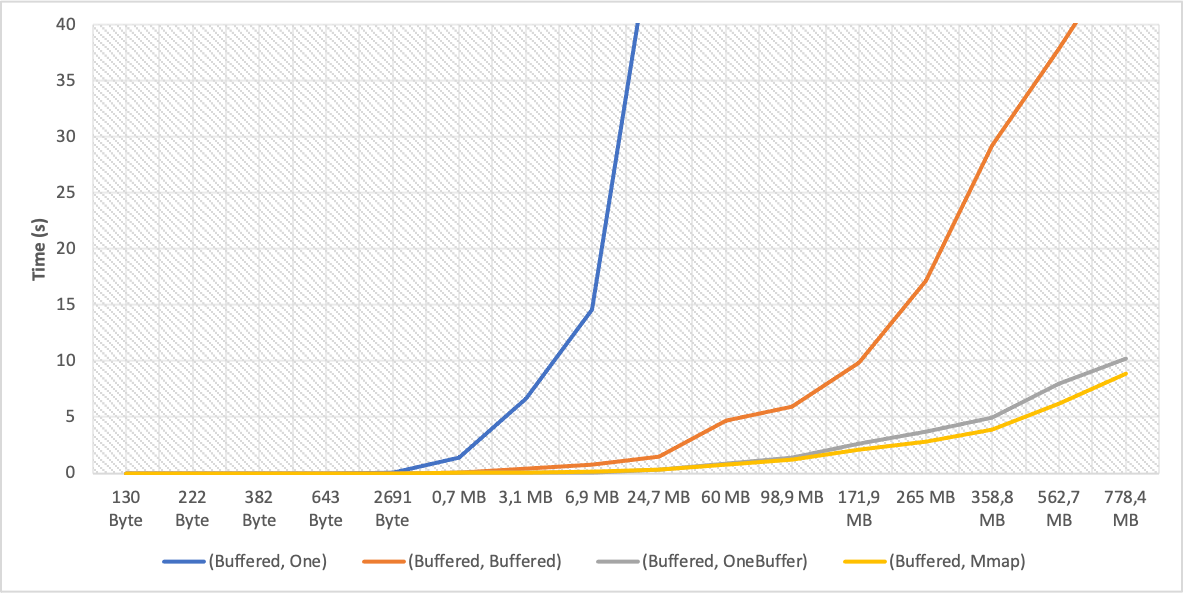
\includegraphics[width=20cm]{images/merge.png}
\end{center}
\caption{RRmerge program using the Buffered input stream}
\label{fig:5}
\end{adjustwidth}
\end{figure}

\begin{figure}[H] 
\begin{adjustwidth}{-3cm}{-1cm}
 \begin{center}
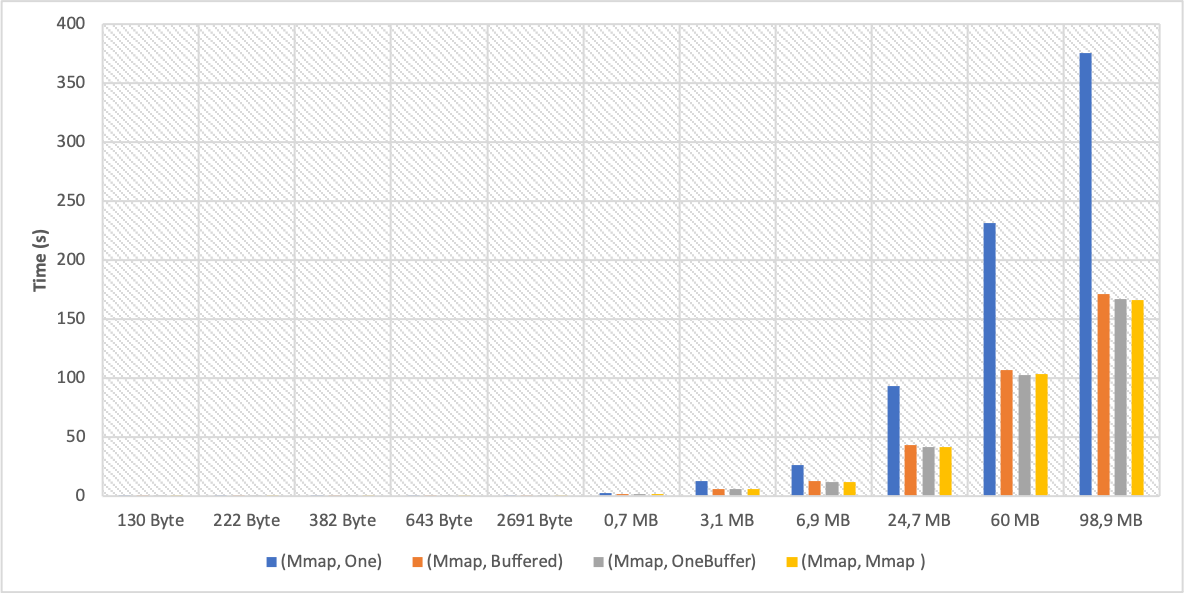
\includegraphics[width=20cm]{images/merge-2.png}
\end{center}
\caption{RRmerge program using the MMap input stream}
\label{fig:6}
\end{adjustwidth}
\end{figure}
\subsubsection{Explanation}
%Explain what you observe.
Globally the results are in agreement with the predictions made the only difference is the top 3 ranking order. The performance of MMap is too bad because it takes a long time for the same case where the Buffered made it in an instant. The output stream One has the worst execution time with the two input streams, and this has been excepted because the writing is done byte by byte, which is more expensive than the other output streams costs. However, this time the MMap outperformed the other output streams and was the best which is not expected because for reading it has the worst execution time. This could be explained by the fact that writing to the buffer immediately effects the changes to the mapped regions of the file. On the other hand, OneBuffer and Buffered have to wait until the buffer is full to commit the changes to the file. Also, the difference between the OneBuffer and the Buffered is noticeable which was not obvious for reading. It is understandable that this difference is due to the size of the buffer which is much bigger than the Buffered one.

\section{Observations on multi-way merge sort}

\subsection{Discussion}

\subsubsection{Expected behavior}
%Explain what kind of performance behavior you expect (before running any experiment) from the implementation. Hereto, define a cost function that estimates the total number of I/Os that need to be done, in function of N, d, and M
Multi-way merge sort is an algorithm that sorts the lines of a file. The lines are sorted by the value of a specific column.

First the algorithm split the main file into multiple sub-files that are sorted by the value of the specific column. These files have approximately the same size $M$ and they are put in a queue. Then the first predefined number $d$ of files are removed from the queue and merged together. The merging is done by reading the current line of each of these files and writing the line in the new output file the one that has the lowest value in the specific column, then the next line is read from the same file. This process stops when the end of every files is reached, then the output file is added to the queue. This operation is done until the queue has $d$ elements or fewer, in which case the operation is done one last time with the remaining files and the result is written in the predefined output file.

At the beginning the input file is split into $B(R) / M$ sorted sublists of $M$ blocks. Then these sublists are merged into larger sublists, still sorted. After this second pass, there are $B(R) / M^2$ sorted sublists of $M'^2$ blocks. After the third pass, $B(R) / M^3$ of $M^3$ blocks. This continues until there are only one sorted sublist left. So, there are $ \lceil \log_{M}B(R) \rceil $ passes. At each pass the entire input is read and written once, $2 B(R)$. Hence the total cost of the multi-way merge is equal to $ 2B(R) \lceil \log_{M}B(R) \rceil $ I/O operations.\\

The estimated overall I/O operation cost is as follows :

\begin{center}
\begin{tabular}{|c|c|}
\hline
\textbf{Implementation} & \textbf{Cost} \\
\hline\hline
One & $ 2B(R) \lceil \log_{M}B(R) \rceil $ \\
[5pt]\hline
Buffered & $ 2\lceil\frac{B(R)}{D}\rceil \lceil \log_{M}\lceil\frac{B(R)}{D}\rceil \rceil $ \\
[5pt]\hline
OneBuffer & $ 2\lceil\frac{B(R)}{S}\rceil \lceil \log_{M}\lceil\frac{B(R)}{S}\rceil \rceil $  \\
[5pt]\hline
MMap & $ 2\lceil\frac{B(R)}{S}\rceil \lceil \log_{M}\lceil\frac{B(R)}{S}\rceil \rceil $ \\
[5pt]\hline
\end{tabular}
\end{center}

For this experiment, only the pair (Buffered, MMap) will be used. Its total cost is as follows : $\lceil\frac{B(R)}{D}\rceil \lceil \log_{M}\lceil\frac{B(R)}{D}\rceil + \lceil\frac{B(R)}{S}\rceil \lceil \log_{M}\lceil\frac{B(R)}{S}\rceil$\\

After estimating the cost, some predictions can be made about the expected parameters tuning results. First the $M$ parameter will be predicted. The increasing of the $M$ parameter should speed up the execution time because it represents the base of the $\log$ in the cost formula. On the other hand, the $d$ and $k$ parameters should not have a considerable influence on the performance, as the number of I/O operations remains the same for any of their values, the only difference would be on the complexity of the sorting algorithm and the resources allocated. The execution time of the algorithm launched on a file and on the sorted version of this file should not be different as the number of I/O operations will still be the same, the only thing that could change is the complexity of the sorting algorithm.

\subsubsection{Implementation}
%Explain the implementation in your own words. Give details on how you programmed the implementation if necessary.
In order to store the files to merge, it has been decided to use a queue containing the input stream linked to each of these files.
To find the lowest value of the specific column in the merging process the use of a priority queue was needed. This priority queue is composed of tuples, one for each of the files to merge. In these tuples the first element is the input stream linked to a file and the second is a list of the value of each column of the current line.
As the files of this project use the \texttt{csv} format, the lines are split and joined with a comma.
The functions \texttt{String.split} and \texttt{String.join} have been used to split the lines in column and to join them again together. 
 
\subsection{Experimental observations}
%Discuss what you observe during your experiments. Use graphs and plots to com- pare the implementations. In each experiment, vary only one parameter (e.g., N) while keeping the other parameters (e.g., M,d) fixed.
For this benchmark the best combination for reading and writing identified in \hyperref[exp1.3]{experiment 1.3} will be used. As seen in \hyperref[res1.3]{experiment 1.3 result} the best pair of input/output streams was (Buffered, MMap). Also, the MMap buffer size was set to 512 kB as in the \hyperref[exp1.3]{experiment 1.3}.\\

First, the value of $M$ will be investigated. Its value will vary while keeping the value of the other variables fixed and random values have been assigned to them. It will vary between three different values : 512 kB, 1 MB and 4 MB. These values will be tested on four different files sorted by their size : ``aka\_title.csv", ``movie\_keyword.csv", ``char\_name.csv" and ``person\_info.csv". The figure \ref{fig:7} shows the execution time of the algorithm with the different values of $M$ on the four different files.

\begin{figure}[H] 
\begin{adjustwidth}{-3cm}{-1cm}
 \begin{center}
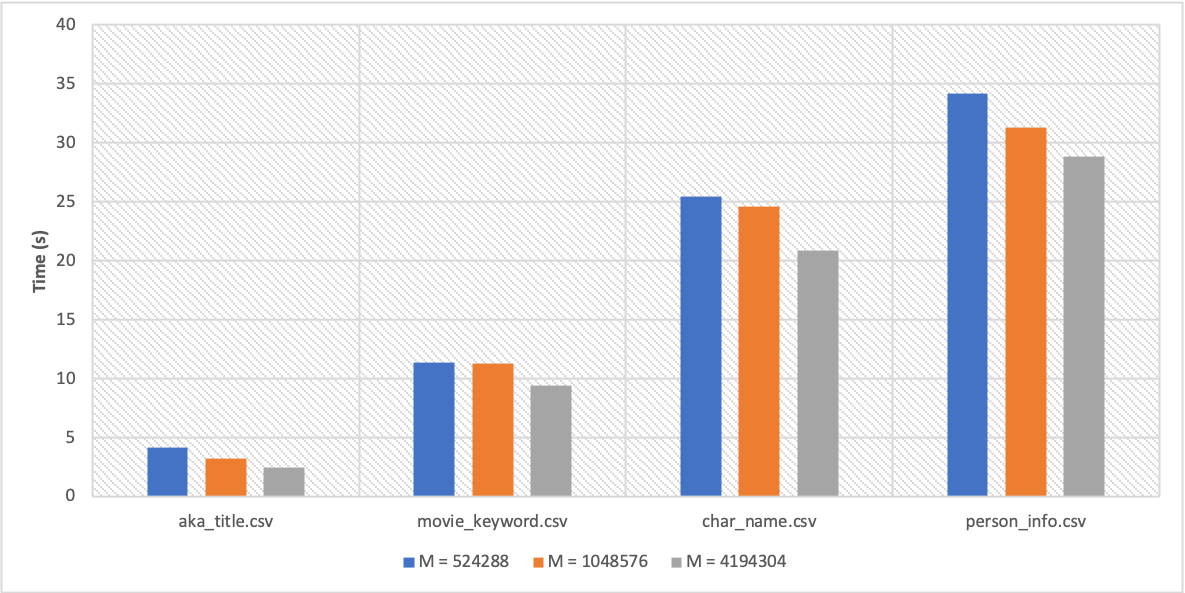
\includegraphics[width=20cm]{images/extsort1.png}
\end{center}
\caption{M parameter tuning}
\label{fig:7}
\end{adjustwidth}
\end{figure}

Next, the value of $d$ will be investigated. Its value will vary while keeping the value of the other variables fixed, the $M$ is set to the best value found in the $M$ parameter tuning experiment. It will vary between eight different values : 5, 10, 15, 20, 25, 30, 35 and 40. These values will be tested on four different files sorted by their size : ``company\_name.csv", ``aka\_name.csv", ``title.csv" and ``name.csv". The figure \ref{fig:8} shows the execution time of the algorithm with the different values of $d$ on the four different files.

\begin{figure}[H] 
\begin{adjustwidth}{-3cm}{-1cm}
 \begin{center}
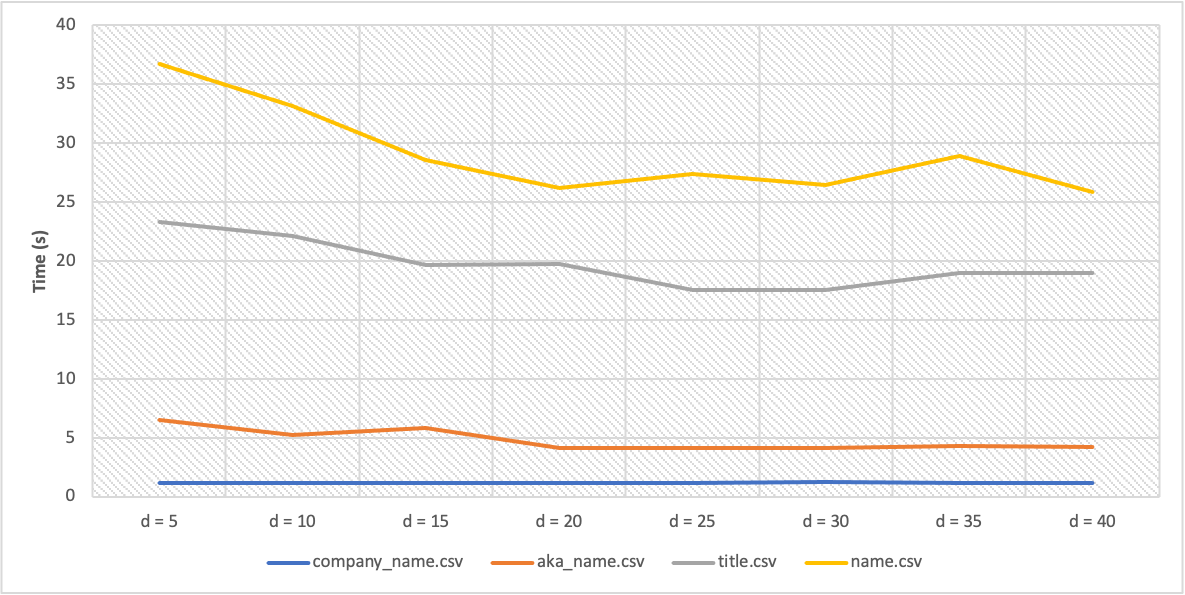
\includegraphics[width=20cm]{images/extsort2.png}
\end{center}
\caption{d parameter tuning}
\label{fig:8}
\end{adjustwidth}
\end{figure}

Then, it will be investigated if there is a difference in execution time when the algorithm sort different columns of the same file. The $M$ and $d$ parameters are set to the best optimal values found during their tuning experiment. The algorithm will be launched on all the columns of four different files : ``keyword.csv", ``movie\_info\_idx.csv", ``movie\_companies.csv" and ``title.csv". The figure \ref{fig:9} shows the execution time of the algorithm on the four different files on all of their columns.

\begin{figure}[H] 
\begin{adjustwidth}{-3.5cm}{-3.5cm}
  \begin{subfigure}[b]{0.5\linewidth}
    \centering
    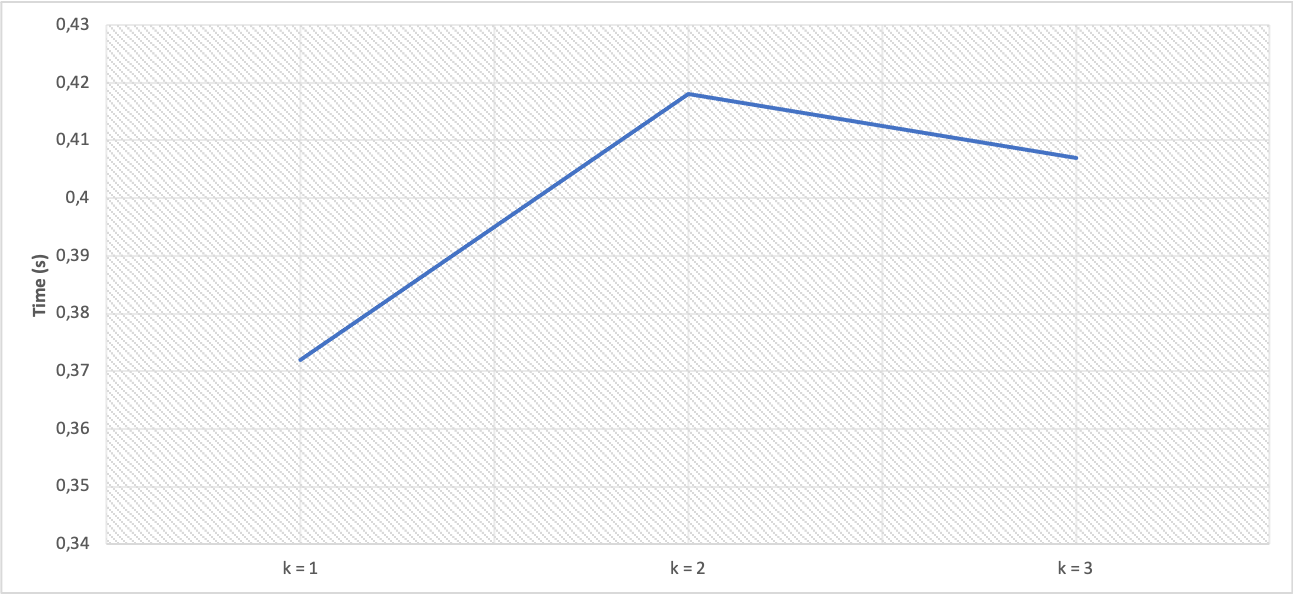
\includegraphics[width=0.99\linewidth]{images/keyword.png} 
    \caption{keyword} 
    \label{fig:9a} 
    \vspace{4ex}
  \end{subfigure}%% 
  \begin{subfigure}[b]{0.5\linewidth}
    \centering
    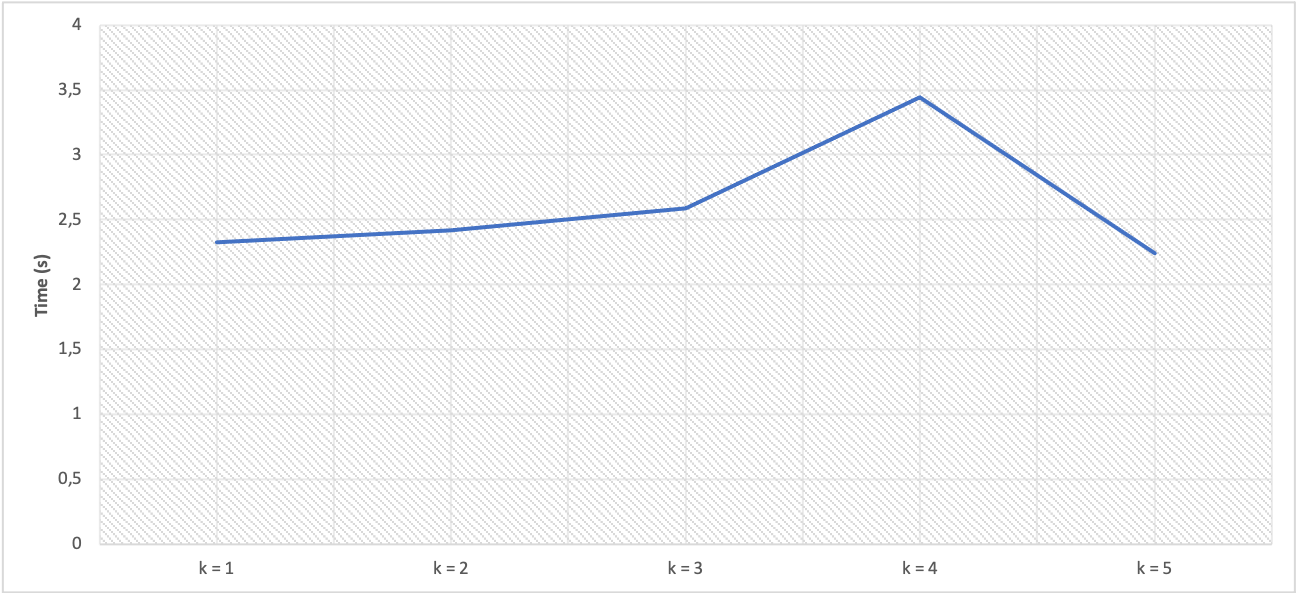
\includegraphics[width=0.99\linewidth]{images/movie_info_idx.png} 
    \caption{movie\_info\_idx} 
    \label{fig:9b} 
    \vspace{4ex}
  \end{subfigure} 
  \begin{subfigure}[b]{0.5\linewidth}
    \centering
    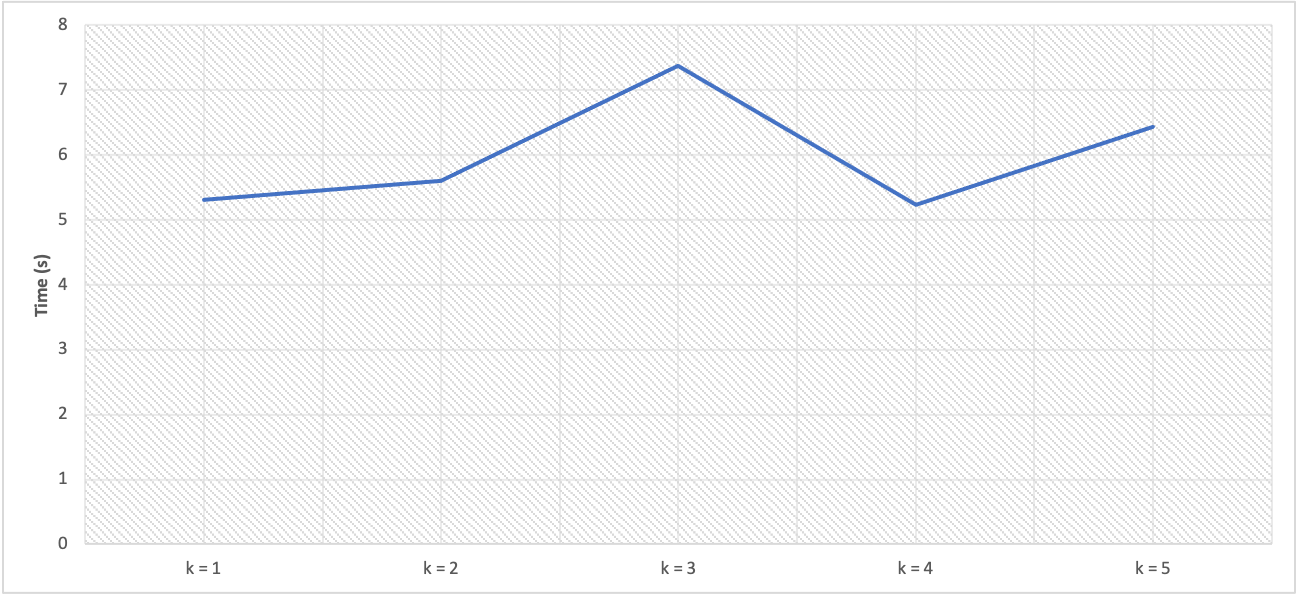
\includegraphics[width=0.99\linewidth]{images/movie_companies.png} 
    \caption{movie\_companies} 
    \label{fig:9c} 
  \end{subfigure}%%
  \begin{subfigure}[b]{0.5\linewidth}
    \centering
    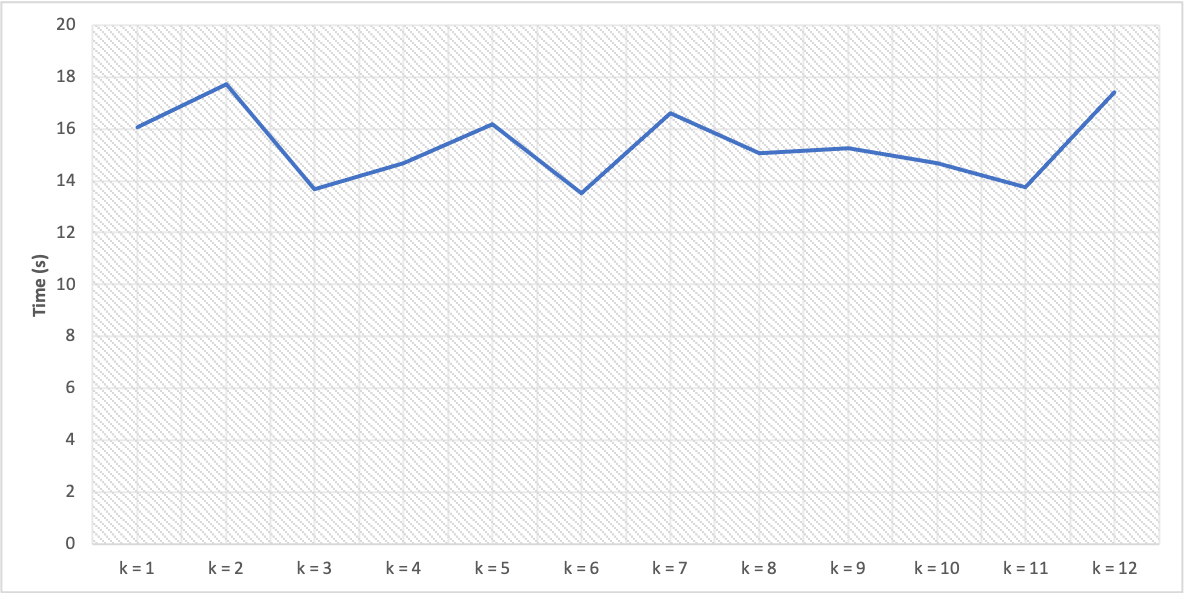
\includegraphics[width=0.99\linewidth]{images/title.png} 
    \caption{title} 
    \label{fig:9d} 
  \end{subfigure} 
  \caption{Files sorts according to different columns}
  \label{fig:9} 
\end{adjustwidth}
\end{figure}

Finally, it will be investigated if there is a difference in execution time when the algorithm is launched on an unsorted file and on a sorted one. The $M$ is set to 4 MB and the $d$ is set to 25 as they are the best values. The algorithm will be launched on the ``cast\_info.csv" file and it will be sorted by the seventh column. The figure \ref{fig:10} shows the execution time of the algorithm when it is launched on the file and on a presorted version of it.

\begin{figure}[H] 
%\begin{adjustwidth}{-3cm}{-1cm}
 \begin{center}
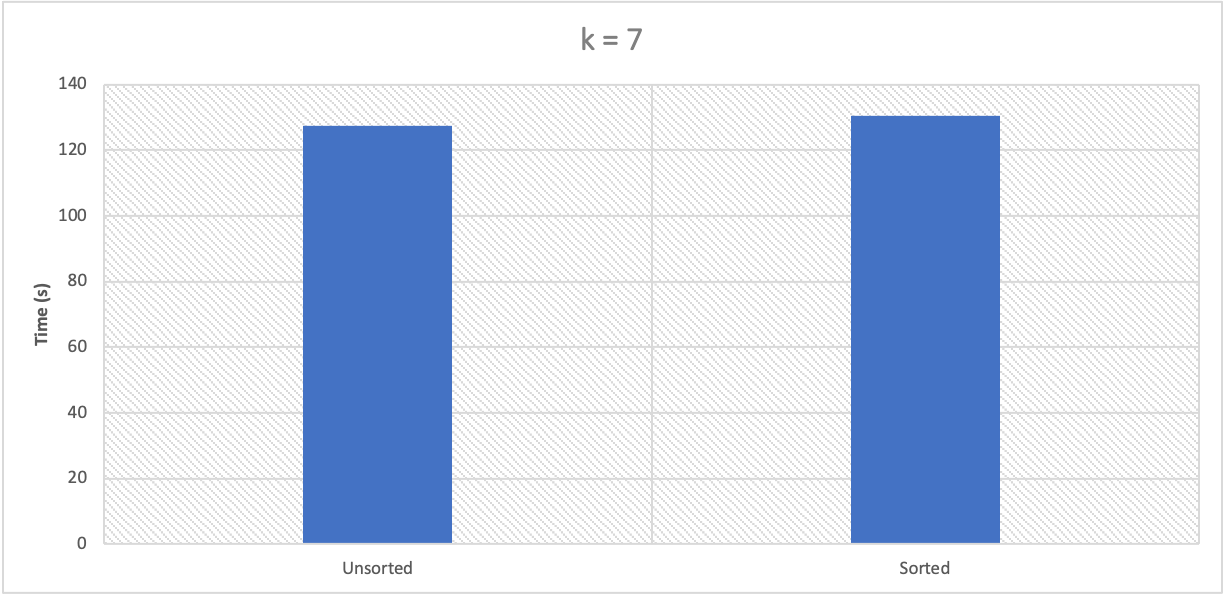
\includegraphics[scale=0.7]{images/sorted-unsorted.png}
\end{center}
\caption{cast\_info}
\label{fig:10}
%\end{adjustwidth}
\end{figure}
\subsection{Explanation}
%Discussion of expected behavior vs experimental observations
%Identify what good choices are of the parameters for varying input sizes.

The prediction is in agreement with the result of the sub-benchmark. The results show that by increasing the value of $M$ the execution time decreases. And that can be explained by the fact that $M$ represent the base of the $\log$ in the cost formula, when the base increases the result decreases. In other words, the number of passes needed decreases as the number of available blocks in the memory increases.

Concerning the $d$ parameter, the result demonstrates that the value of $d$ for small files does not affect their execution time, but it does for bigger files. Globally there is not an optimal value for $d$ as the execution time fluctuate in the same interval. And it comes down to the fact that the number of I/O operations needed does not depends on $d$ as the file will be read and written entirely but it will change the number of temporary files to create. When $d$ increases the number of temporary files decreases but the size of the memory that the program needs also increases as there are at most $\mathcal{O}(d)$ lines in memory.

About the $k$ parameter, the result confirms what was expected as there are no big differences in the execution times. Files sorts according to different columns have no impact on the execution time of the algorithm. As the main memory sorting algorithm has almost the same performance because $O(d)$ in the test circumstances does not create a big difference for the complexity time of the algorithm.

As expected, the execution time of the algorithm on a file and on a sorted version of this file stays the same. This is due to the fact that the number of I/O operations the algorithm does not change because of the order of the lines as the length of the lines stays the same. The main memory algorithm does not know that the elements are already sorted so it will try to sort them, that means that the time complexity stays the same.

\section{User manual}
In the root folder of this project a \texttt{pom.xml} file has been added. This file follows the Maven Java structure. It allows to build the project and generate the benchmarks executable. All the result that were used in this report will be available in the \texttt{benchmark-logs} folder. In order to be able to reproduce them the following procedure should be followed.

\begin{lstlisting}[language=bash]
  $ mvn clean
  $ mvn package
\end{lstlisting}

Once theses commands have been executed, a new directory named \texttt{target} will appear. This directory contains the executable.

When executing the benchmark jar, all the benchmarks are launched (which can take a while). To specify one benchmark only the name of the class is needed.

The command line can be as follow :

\begin{itemize}

\item To launch all the benchmarks of the OneBuffer (i.e. length, randjump):
\begin{lstlisting}[language=bash]
  $ java -jar target/benchmarks.jar OneBuffer
\end{lstlisting}

\item To launch the benchmarks of the length program with the OneBuffer implementation:
\begin{lstlisting}[language=bash]
  $ java -jar target/benchmarks.jar OneBuffer.length
\end{lstlisting}

\item To launch the benchmarks of the length program with the OneBuffer with a fixed BufferSize parameter :
\begin{lstlisting}[language=bash]
  $ java -jar target/benchmarks.jar OneBuffer.length -p BufferSize=1024
\end{lstlisting}

\item To launch the benchmarks of the extsort program with a fixed input stream, a fixed output stream and $k$ that takes the value 2 then 5 (there should only be commas in all the values the parameter should take, no space) :
\begin{lstlisting}[language=bash]
  $ java -jar target/benchmarks.jar extsort -p xPair=Buffered -p yPair=Mmap -p k=2,5
\end{lstlisting}

\end{itemize}

\section{Conclusion}
%Summarize what you have learned in this project.

In this project four implementations of input/output have been done. By implementing them, it shows how files can be manipulated. Their performances have been observed over several experiments. It has been shown that each of these implementations have their strengths and their weaknesses, there is no perfect input or output streams for all cases. For example, when reading sequentially a file, the Buffered and the One buffer have demonstrated their superiority but in random reading the MMap showed its dominance. As it has been seen, the implementation using an in-memory buffer have always the best execution times. These two experiments have shown that the chosen input stream should be selected according to the use case to have the best performance.

Another concept learned in the project was the memory mapping. As opposed to the traditional input/output implementations, it does not use the RAM. It allows the manipulation of files directly through the dynamic memory.

It has been shown that the combining of two different types of streams for the input and output one is beneficial to obtain the best performance. As seen the pair (Buffered, MMap) and the pair (Buffered, OneBuffer) offer great performance compared to any other pairs.

The last experiment gave a real-world experience with the performance of an important external-memory algorithm, multiway merge, which sorts the lines of the files. The tuning of the different parameters allowed the finding of the optimal values for each of them.

The time complexity of the used algorithm is important, but number of I/O operations is also a value to take into account. The performances obtained on one machine might differ from the one obtained on another one, especially if the type of the secondary memory is not the same in the case of this project.

\end{document}